\section{Results}\label{sec:results}

\subsection{The two maps}

Figure~\ref{fig:maps} shows the two 2-D PCA maps with identical plotting settings. Map A's leading components are brightness gradients, with 23.8\% of pixel variance in component~0 and 2, 4, 19, and 66 components for 25\%, 50\%, 75\%, and 90\% (95\% not reached in the first 100); Map B needs 3, 7, 15, 24, and 31, and its first component carries 10.9\%. Map A's 2-D axes are illumination: PC1 is a brightness axis ($r=0.986$ with mean image brightness) and PC2 a lateral gradient ($r=0.944$); the lobes are brightness groups, not identities.

The crucial check is the rank correlation between 2-D and full-dimensional pairwise distances: Map A's plot preserves more of its space's geometry ($\rho=0.807$) than Map B's plot preserves of the embedding space ($\rho=0.517$). The embedding is the better representation; its 2-D picture is the less faithful one. Figure~\ref{fig:components} shows the eigenfaces and variance curves. The projections are stable across seeds 0--2, while full-dimensional metrics are deterministic.

\begin{figure}[t]
\centering
\begin{subfigure}[t]{0.44\textwidth}
  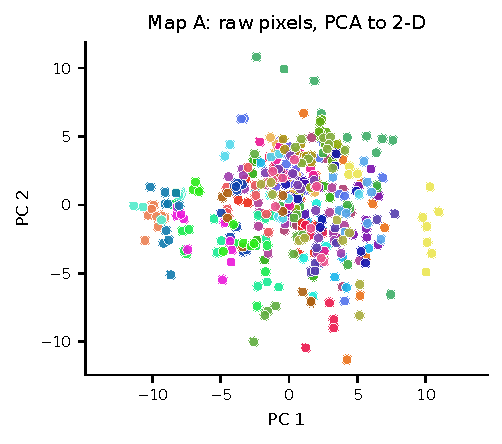
\includegraphics[width=\linewidth]{mapA_scatter.pdf}
  \caption{Map A: raw pixels.}
\end{subfigure}\hfill
\begin{subfigure}[t]{0.44\textwidth}
  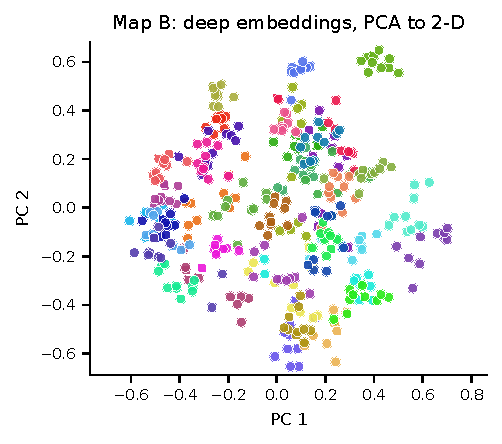
\includegraphics[width=\linewidth]{mapB_scatter.pdf}
  \caption{Map B: frozen embeddings.}
\end{subfigure}
\caption{The two 2-D maps with identical colour, axis, and PCA conventions. Presentation only: every metric is computed on the full 4096-d and 512-d vectors. The raw-pixel map preserves more pairwise geometry (rank correlation 0.807) than the embedding map (0.517), even though the embedding is the better representation.}
\label{fig:maps}
\end{figure}

\begin{figure}[t]
\centering
\begin{subfigure}[t]{0.4\textwidth}
  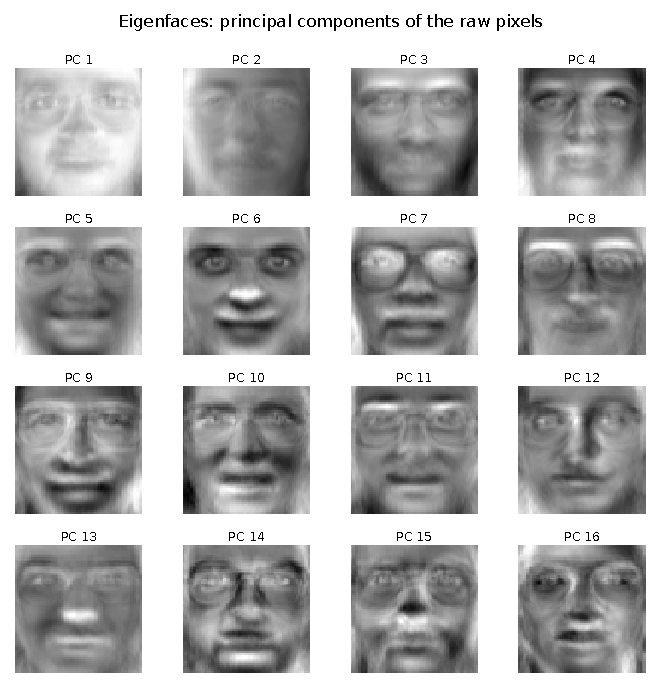
\includegraphics[width=\linewidth]{eigenfaces.pdf}
  \caption{First 16 Eigenfaces.}
\end{subfigure}\hfill
\begin{subfigure}[t]{0.53\textwidth}
  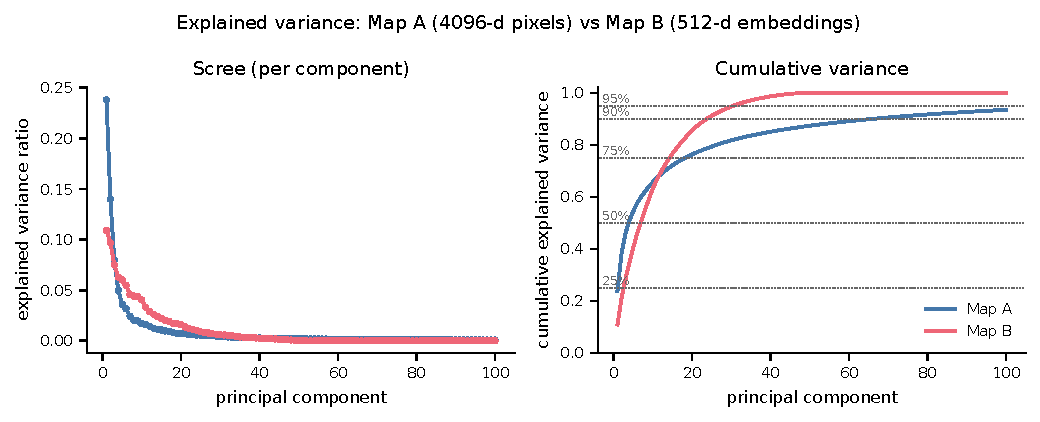
\includegraphics[width=\linewidth]{scree.pdf}
  \caption{Explained and cumulative variance.}
\end{subfigure}
\caption{Map A's leading components are illumination and low-frequency shape patterns, not identity features; component~0 alone carries 23.8\% of the raw-pixel variance. Map B's variance is spread over more components (31 for 95\%) than Map A's concentrated variance.}
\label{fig:components}
\end{figure}

\subsection{Quantitative comparison}

Table~\ref{tab:main} gives the full-dimensional comparison; every row favours the embedding. Silhouette more than quadruples, 1-NN accuracy reaches 100\% from 94.5\%, pair ROC-AUC rises from 0.881 to 0.9995, pair EER falls from 20.5\% to 1.11\%, and $d'$ roughly triples. Map A's genuine distances ($8.38\pm2.56$) overlap heavily with its impostors ($12.41\pm2.45$), while Map B's are nearly disjoint ($0.53\pm0.19$ versus $1.33\pm0.13$; Figure~\ref{fig:hist-roc}). The matched-dimensionality control (399 components, 100\% variance retained) reproduces Map A's metrics exactly (silhouette 0.10557, AUC 0.8807, EER 0.2050; maximum distance difference $3.5\times10^{-12}$), so the gaps are not dimension artefacts.

\begin{table}[t]
\centering
\caption{Main comparison in full dimensionality. Pair-level metrics use all 1,800 genuine and 78,000 impostor pairs from the 400 Olivetti images. The 399-component dimensionality control reproduces every Map A row to numerical precision.}
\label{tab:main}
\footnotesize
\begin{tabular}{@{}lcc@{}}
\toprule
Metric & Map A: raw pixels (4096-d) & Map B: embedding (512-d) \\
\midrule
Silhouette (40 identities) & 0.1056 & \textbf{0.4970} \\
1-NN leave-one-out accuracy & 0.9450 & \textbf{1.0000} \\
1-NN leave-one-out top-5 & 0.9825 & \textbf{1.0000} \\
Pair ROC-AUC & 0.8807 & \textbf{0.99954} \\
Pair EER & 0.2050 & \textbf{0.01111} \\
TAR at FAR $=10^{-3}$ & 0.2639 & \textbf{0.9550} \\
TAR at FAR $=10^{-2}$ & 0.4233 & \textbf{0.9883} \\
$d'$ & 1.612 & \textbf{4.988} \\
Genuine distance (mean $\pm$ sd) & $8.378\pm2.556$ & $0.5284\pm0.1860$ \\
Impostor distance (mean $\pm$ sd) & $12.414\pm2.450$ & $1.3336\pm0.1324$ \\
2-D rank correlation & \textbf{0.8070} & 0.5174 \\
\bottomrule
\end{tabular}
\end{table}

\begin{figure}[t]
\centering
\begin{subfigure}[t]{0.44\textwidth}
  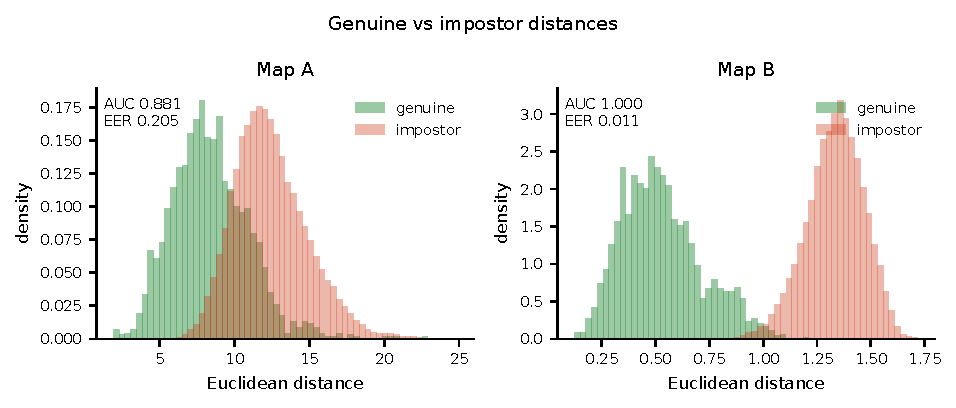
\includegraphics[width=\linewidth]{distance_histograms.pdf}
  \caption{Genuine and impostor distances.}
\end{subfigure}\hfill
\begin{subfigure}[t]{0.44\textwidth}
  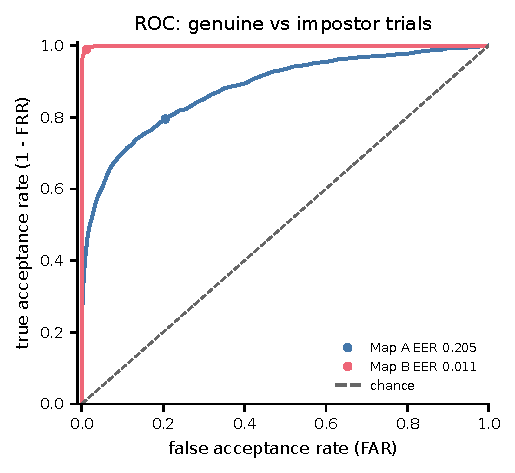
\includegraphics[width=\linewidth]{roc_curves.pdf}
  \caption{Pair-level ROC with EER.}
\end{subfigure}
\caption{Pair-level verification. Map A's distributions overlap substantially; Map B's are nearly disjoint. Curves use the same 1,800 genuine and 78,000 impostor distances, not the 2-D maps.}
\label{fig:hist-roc}
\end{figure}

\subsection{Why the metrics disagree}

Raw pixels look respectable on identification (94.5\% 1-NN) but poor on silhouette (0.106 versus 0.497) and worse on open-set verification (EER 8.7\% versus 0.22\%). Identification asks whether the single nearest gallery image is correct, and with ten images per identity and pre-aligned data it often is. Verification fixes one threshold and requires the distributions to be separated, not merely ordered; Map A's overlap makes that impossible, Map B's near-disjoint distributions make it easy. A good nearest-neighbour result is not evidence that a face-unlock threshold exists. The maps agree on 378 of 400 predictions (94.5\%), Map B makes no errors, and there is no ``both wrong'' set (reported as \texttt{null}, not zero). Figure~\ref{fig:diagnostics} summarises the metric gaps and per-identity accuracy.

\begin{figure}[t]
\centering
\begin{subfigure}[t]{0.53\textwidth}
  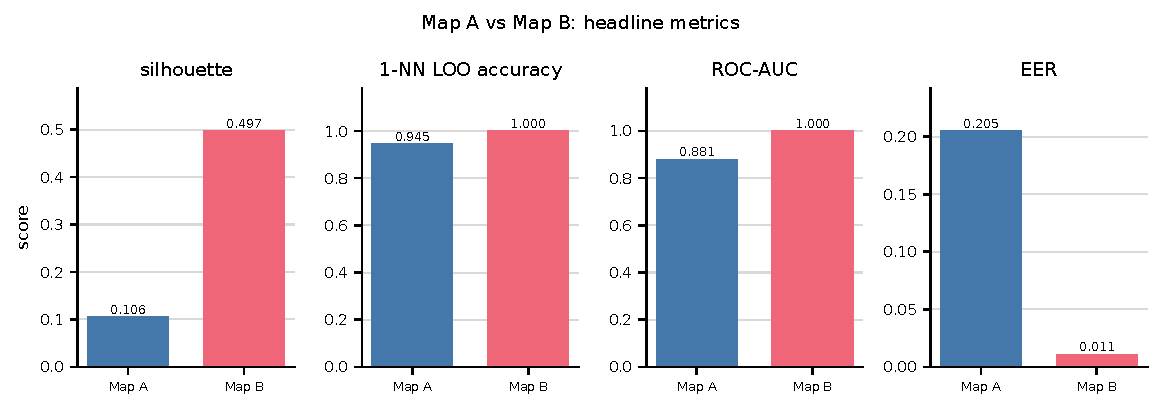
\includegraphics[width=\linewidth]{metric_bars.pdf}
  \caption{Metric summary.}
\end{subfigure}\hfill
\begin{subfigure}[t]{0.4\textwidth}
  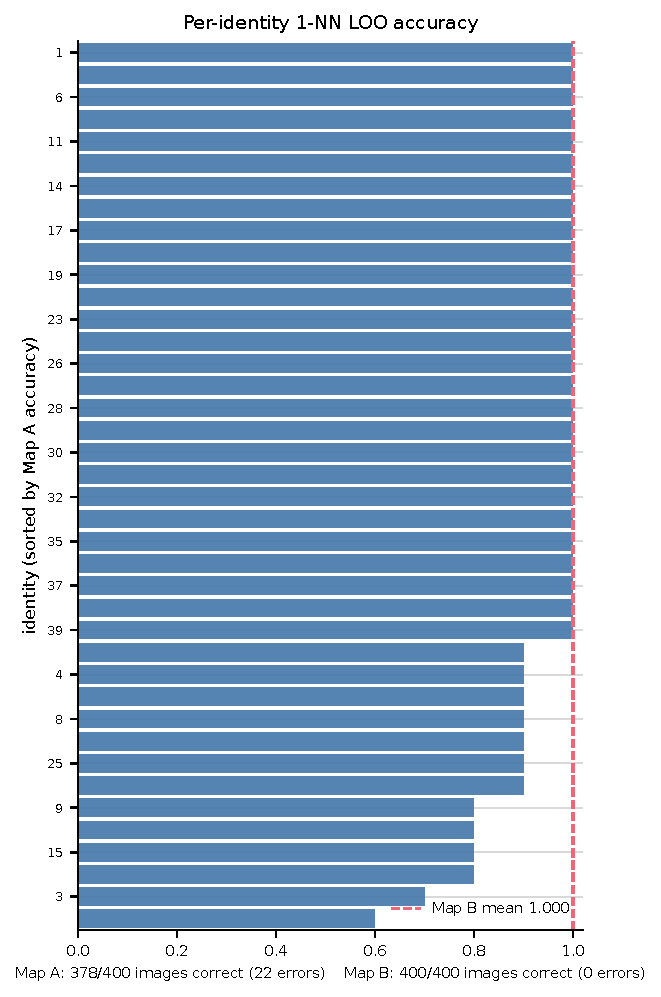
\includegraphics[width=\linewidth]{confusion_panel.pdf}
  \caption{Per-identity 1-NN accuracy.}
\end{subfigure}
\caption{Metric summary and per-identity accuracy. The embedding wins every metric; Map B is perfect on every identity, while Map A's errors concentrate in a few identities. Cross-map prediction agreement is 94.5\%.}
\label{fig:diagnostics}
\end{figure}

\subsection{Open-set verification and the threshold dial}

Table~\ref{tab:operating} reports the FaceID-style protocol. Map A's EER is 8.71\% (sd 1.25 points) and Map B's is 0.22\% (sd 0.24 points). Map B's figure is at or below the protocol's 0.5\% FRR resolution (200 genuine trials per split), so read it as ``at the measurement floor''; the roughly 39-fold EER ratio inherits that floor. The matched-FRR comparison is not floor-limited (15,600 impostor trials per split, FAR resolution 0.0064\%): at 1\% false-reject rate, Map A accepts 48.59\% of impostors and Map B 0.044\%, roughly 1,115 times fewer for Map B. At a 1\% false-accept rate, Map B accepts 99.9\% of genuine probes versus 74.6\% for Map A.

Figure~\ref{fig:threshold-curves} shows the curves on separate axes: the EER thresholds are 8.505 and 0.8396, roughly ten times apart, and a shared axis would invite a false comparison of threshold values. Map A has no threshold with both error rates small; Map B has a broad operating region. Robustness checks do not change the ranking: the fixed first-half/second-half split gives EERs 9.00\% and 0.256\%, the mean-template rule 11.85\% and 0.22\%. Pair-level EERs (20.5\% and 1.11\%) are a different protocol and agree on ranking, not absolute value; the open-set protocol supplies the headline numbers.

\begin{table}[t]
\centering
\caption{Open-set verification: five random 5/5 splits (seeds 0--4), 200 genuine and 15,600 impostor trials per split. Scores are minimum distances to the five enrolment images; accept if score $\le\tau$. Mean (sd) across splits. Map B's EER is at the protocol's 0.5\% FRR resolution.}
\label{tab:operating}
\footnotesize
\begin{tabular}{@{}lcc@{}}
\toprule
Operating point & Map A & Map B \\
\midrule
EER & 0.0871 (0.0125) & 0.00224 (0.00244) \\
EER threshold & 8.505 & 0.8396 \\
TAR at FAR $=10^{-3}$ & 0.593 & 0.994 \\
TAR at FAR $=10^{-2}$ & 0.746 & 0.999 \\
FAR at matched FRR $=1\%$ & 0.4859 (0.1189) & 0.000436 (0.000378) \\
AUC & 0.96999 & 0.99997 \\
\bottomrule
\end{tabular}
\end{table}

\begin{figure}[t]
\centering
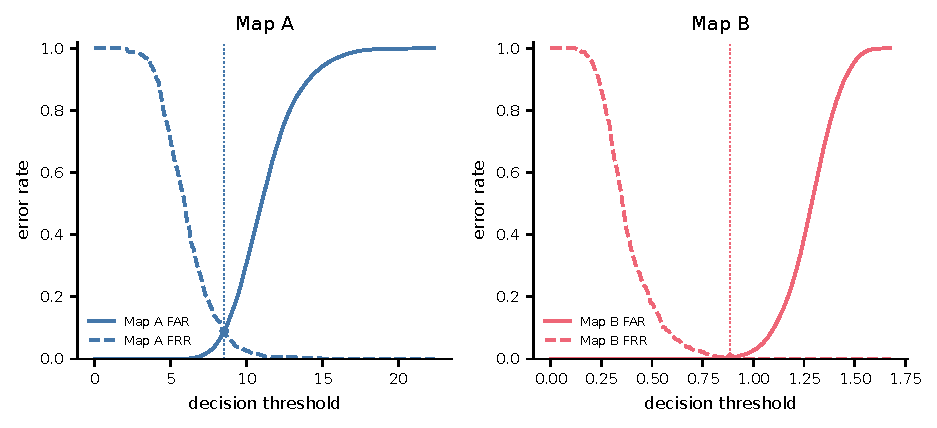
\includegraphics[width=0.476\textwidth]{threshold_curves.pdf}
\caption{FAR (solid) and FRR (dashed) against threshold, with EER marked. Separate axes are used because the representations produce distances on different scales (EER thresholds 8.505 versus 0.8396). Map A has no threshold with both error rates small; Map B has a wide operating region.}
\label{fig:threshold-curves}
\end{figure}

\subsection{Webcam illumination study}

Table~\ref{tab:lighting} summarises the study. The frame-to-frame noise floor is 0.186 (per-scan means 0.114--0.334), and same-condition repeats differ by 0.227--0.371. Changing the \emph{amount} of light moves the mean distance to 0.258 (range 0.168--0.384), inside the repeat-scan range: brightness is effectively free. Changing the \emph{direction} moves it to 0.714, 3.83 times the noise floor. Front-to-side pairs are large (0.636--0.733) while left--right is smaller (0.511), so two half-shadowed faces resemble each other more than either resembles a front-lit face---a ``half-shadowed'' region. Side-to-bottom is worst (0.808--0.888), consistent with under-lighting being rare in photographic training data. Pooling frames reduces mean distances by 4.82\% (0.604 to 0.575), a modest gain that does not change condition ordering (Figure~\ref{fig:live}).

The worst same-person pair is flash/right repeat~2 against flash/bottom repeat~2: 0.967 frame-level (cosine similarity 0.532, cosine distance 0.468), 0.915 after scan averaging (cosine similarity 0.581, cosine distance 0.419). A frame-level threshold below 0.967 would reject the enrolled user in at least one observed condition; a scan-mean threshold below 0.915 would do so. That is the convenience side of the dial, measured on one person. Frames are not independent (mean within-scan distance grows from 0.153 at lag~1 to 0.257 at lag~9), so the effective sample size per scan is below ten; frame~0 is also a warm-up outlier (0.243 versus 0.167 at frame~5).

\begin{table}[t]
\centering
\caption{Webcam illumination study summary (Euclidean distances between unit-norm embeddings; cosine similarity $=1-d^2/2$). The noise floor is the mean within-scan frame-pair distance over twelve scans. The worst genuine pair is flash/right repeat~2 versus flash/bottom repeat~2. The cross-domain row is domain-confounded and is an upper bound only.}
\label{tab:lighting}
\footnotesize
\begin{tabular}{@{}lc@{}}
\toprule
Quantity & Value \\
\midrule
Within-scan jitter (noise floor) & 0.186 \\
Same-condition between-scan means & 0.227--0.371 \\
Intensity effect (room/front vs flash/front) & 0.258 \\
Direction effect (six flash direction pairs, mean) & 0.714 \\
Direction / noise ratio & 3.83 \\
Pooling reduction (scan means vs frames) & 4.82\% \\
Worst genuine frame pair & 0.967 \\
Worst genuine after scan averaging & 0.915 \\
Cross-domain minimum (Olivetti to live scan) & 0.887 \\
\bottomrule
\end{tabular}
\end{table}

\begin{figure}[t]
\centering
\begin{subfigure}[t]{0.32\textwidth}
  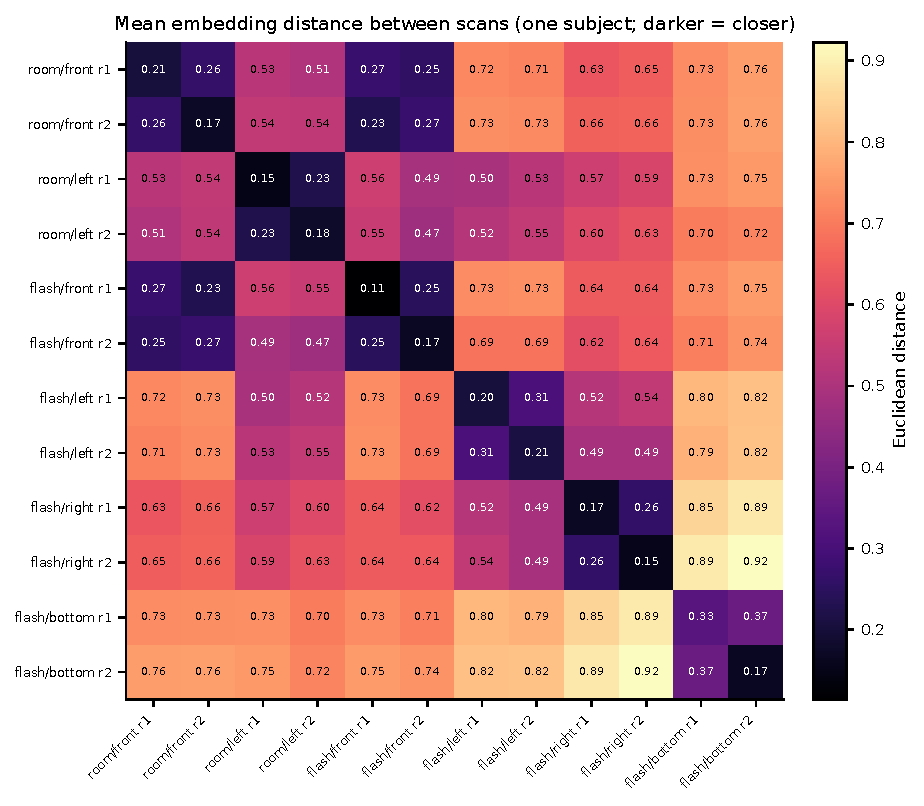
\includegraphics[width=\linewidth]{live_heatmap.pdf}
  \caption{12$\times$12 scan distances.}
\end{subfigure}\hfill
\begin{subfigure}[t]{0.28\textwidth}
  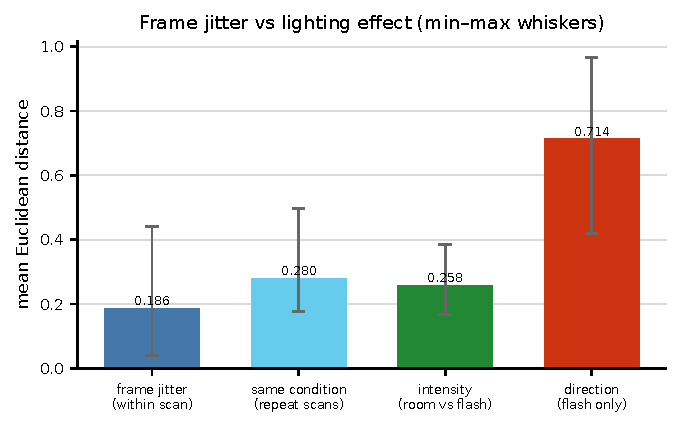
\includegraphics[width=\linewidth]{live_lighting.pdf}
  \caption{Noise floor, intensity, direction.}
\end{subfigure}\hfill
\begin{subfigure}[t]{0.28\textwidth}
  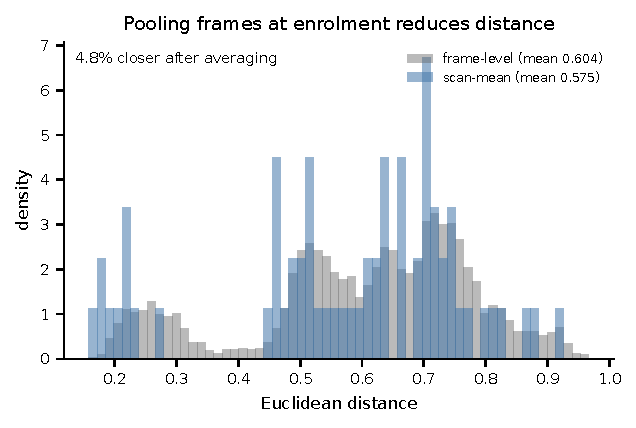
\includegraphics[width=\linewidth]{live_pooling.pdf}
  \caption{Frame-level vs scan means.}
\end{subfigure}
\caption{Live illumination study. Repeat scans of the same condition are close and condition blocks are separated by roughly the direction effect; brightness changes are indistinguishable from repeat-scan noise, while direction changes are about four times the frame-to-frame noise floor. Pooling ten frames into a scan mean reduces distances modestly and does not remove the direction effect.}
\label{fig:live}
\end{figure}

The smallest distance from any Olivetti embedding to any live scan is 0.887 (frame-level 0.880; mean of per-Olivetti minima 1.288). It is domain-confounded---different capture device, crop, resolution, and people---so it is an upper bound only, not a calibrated impostor distribution (Section~\ref{sec:discussion}).
